\chapter{Structural Properties of Non-KM-forcing Graphs}
\label{chap:structural-properties}

We earlier saw in section~\ref{section:rooted-minors} results implying the existence of rooted minors, where some connectivity constraints were assumed.
Therefore, it is natural to think that connectivity of a graph $G$ might play a role in determining whether a given graph $H$ is KM-forced in $G$.

By Theorem \ref{thm:5}, all graphs with five vertices and, at most, six edges are KM-forcing.
We aim to investigate the connectivity properties of graphs \( G \) where some graph \( H \) is non-KM-forced.
By the following lemma, which proves a stronger statement, we will show that if \( H \) has at least seven edges and five vertices, and there exists some graph \( G \) in which \( H \) is non-KM-forced, then smallest such \( G \) is 2-connected.

\begin{lemma}
   \label{main-lemma}
 Let $H$ and $G$ be graphs, let $\mathfrak{C}$ be a coloring of $G$, and let $T$ be the corresponding transversal such that
   $H$ is isomorphic to $H(G, \mathfrak{C}, T)$.
   
 Suppose the following hold:
   \begin{enumerate}[label=(\arabic*)]
      \item $H(G, \mathfrak{C}, T)$ is not a $T$-rooted minor in $G$.
      \item Every proper subgraph $H'$ of $H$ is KM-forcing.
      \item If $H$ is non-KM-forced in any other graph $G' \ncong G$, then
     $$|V(G)| + |E(G)| \leq |V(G')| + |E(G')|.$$
   \end{enumerate}
 Then $G$ is 2-connected.
\end{lemma}
   
   \begin{proof}

 Graph $H$ is connected, since if it were not, by condition (2) we would have that every component of $H$ is KM-forcing, and by theorem~\ref{thm:1.5}  we would conclude that $H$ is KM-forcing, which is a contradiction. 
   
 Every vertex from $V(H)$ has degree at least 2, since if some of the vertices have 
 degree 1, then by theorem~\ref{thm:2} and condition (2) we would conclude that $H$ is KM-forcing, which is again a contradiction.

 Condition (3) forces $G$ to be a minimal such graph with properties (1) and (2). 
 By minimality of $G$, for each pair of distinct color classes $A, B \in \mathfrak{C}$, 
 the subgraph of $G$ induced by $ A\cup B$ is a set of isolated vertices and a single path connecting the corresponding transversal 
 vertices in $T$.
   
 Assume, for contradiction, that $G$ is not 2-connected. Then $G$ is either disconnected or 1-connected.

 If $G$ is disconnected, since $H$ is connected, then the transversal vertices are in the same component of $G$, but then condition (3)
 doesn't hold, since we can have smaller graph $G'$ which is the component where $H$ is non-KM-forced.

 If $G$ is 1-connected, then by definition, there exists a cut vertex $x$
 splitting $G$ into two subgraphs $L$ and $R$ that intersect only at $x$ (see Figure~\ref{fig:general-case}).

    \begin{figure}[h]
      \centering
      \vspace{0.3cm}
      
\includegraphics[width=6cm]{img/general-case.eps}
      \vspace{0.3cm}
      \caption{A cut vertex $x$ splitting $G$ into subgraphs $L$ and $R$.}
      \label{fig:general-case}
  \end{figure}
   
   \textbf{Case 1: $x \in T$ i.e it is a transversal vertex.}
   
 No transversal vertex in $V(L \setminus \{x\})$ can connect to one in $V(R \setminus \{x\})$ via a Kempe chain. Because
$x$ is a cut vertex, such a chain must pass through $x$. However, the Kempe chain between two distinct
 color classes would contain another color class of $x$, which is impossible. By condition (3),  
 any Kempe chain between $x$ and another transversal vertex is either fully contained in $L$ or $R$. Hence, no Kempe chain between the transversal vertices
 can cross the cut vertex $x$. 
   
 Let $T_L$ be the transversal vertices from subgraph $L$, and let $H_L$ be the subgraph of $H(G, \mathfrak{C}, T)$ induced by $T_L$.
 Let $T_R$ and $H_R$ be defined similarly for $R$. By condition (2), 
 both $H_L$ and $H_R$ are KM-forcing in the corresponding subgraphs of $G$, 
 so there is a $T_L$-rooted minor of $H_L$ in $L$ and a $T_R$-rooted minor of $H_R$ in $R$. 
 Since the bags of models of $H_L$ in $L$ and $H_R$ in $R$ contain disjoint vertex sets (except $x$) and respect the transversal roots, 
 combining them results in a $T$-rooted minor of $H(G, \mathfrak{C}, T)$ in $G$, contradicting condition (1).
   

\textbf{Case 2: $x \not\in T$ i.e $x$ is not a transversal vertex.}
   
 If no Kempe chain passes through $x$ between $L$ and $R$, the same argument as in Case 1 applies.
 Otherwise, suppose there is a Kempe chain from $L$ passing through $x$ to $R$. 
 Let $a$ be the end vertex of the Kempe chain in $L$ and $b$ be the end of the Kempe chain in $R$. Both $a$ and $b$ are transversal vertices by condition (3).
 WLOG $x$ has the color of $b$.

 Let $H_L$ be the subgraph of $H(G, \mathfrak{C}, T)$ induced by the vertices $(V(L) \cap T) \cup \{b\}$. Let $\mathfrak{C}_L$ be the coloring of $L$ induced by the coloring $\mathfrak{C}$.
 Let $T_L := (V(L) \cap T) \cup \{x\}$ be the transversal of the coloring $\mathfrak{C}_L$. Since $x$ has color of the transversal vertex $b$ in $G$, all relevant Kempe chains corresponding to the 
 edges of $H_L$ remain in $L$, therefore $H_L$ is isomorphic to $H(L, \mathfrak{C}_L, T_L)$. By condition (2), $H(L, \mathfrak{C}_L, T_L)$ is a $T_L$-rooted minor in $L$.
   
 Let $H_R$ be the subgraph of $H(G, \mathfrak{C}, T)$ induced by the vertices $(V(R) \cap T) \cup \{a\}$. $H_R$ is a proper subgraph of $H(G, \mathfrak{C}, T$),
otherwise there is only one Kempe chain from $L$ to $R$ and the degree of $a$ is one in $H$; by theorem~\ref{thm:2} and condition (2) we would conclude that $H$ is KM-forcing, which is a contradiction. 
 Let $R'$ be the graph formed from $R$ by adding a single edge from $x$ to a new vertex $a$ as shown in figure~\ref{fig:case2-2-connectedness}. 
 Let $\mathfrak{C}_R$ be the coloring of $R'$ induced by the coloring $\mathfrak{C}$. Let $T_R := (V(R') \cap T)$ be the transversal of the coloring $\mathfrak{C}_R$
 By the construction of $H_R$, the Kempe chains in $R'$ correspond to edges of $H_R$, hence $H_R$ is isomorphic to $H(R', \mathfrak{C}_R, T_R)$. 
 By condition (2), $H(R', \mathfrak{C}_R, T_R)$ is a $T_R$ rooted minor in $R'$.
   
 \begin{figure}[h]
  \centering
  \vspace{0.2cm}
  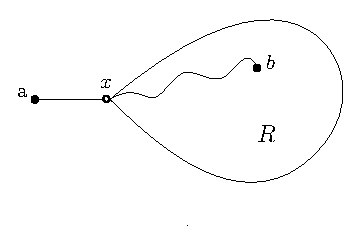
\includegraphics[width=6cm]{img/case2-2-connectedness}
  \vspace{0.2cm}
  \caption{$R'$}
  \label{fig:case2-2-connectedness}
\end{figure}

The models of the rooted minors of $H_L$ in $L$ and $H_R$ in $R'$ have a common color as a root with the color of $a$. If we can show that 
there is a model of $H_R$ in $R'$ where the bag $B_a$ only contains a single vertex i.e $B_a = \{a\}$, then we can combine the models of $H_L$ and $H_R$ to get a model of $H(G, \mathfrak{C}, T)$ in $G$. 

We concluded earlier that each vertex of $H$ has a degree of at least 2; hence, all the Kempe chains $G$ passing through $x$ from $L$ to $R$ are connected to $b$. 
Hence, $a$ is connected to only $b$ from the transversal vertices from $V(R) \cap T$. So we can extend the bag $B_b$ of the model of $H_R$ in $R'$ to include $x$.
This means we have a valid model of $H_R$ in $R'$ where the bag $B_a$ only contains a single vertex, i.e, $B_a = \{a\}$.

Now we can combine the models of $H_L$ in $L$ and $H_R$ in $R'$ to get a model of $H(G, \mathfrak{C}, T)$ in $G$.
   
 In all cases, we reach a contradiction. Therefore, $G$ must be 2-connected.
   \end{proof}

\begin{cor}
Let $H$ be a graph on five vertices and at least seven edges.
Let $G$ be a graph with coloring $\mathfrak{C}$ and transversal $T$ such that $H$ is isomorphic to $H(G, \mathfrak{C}, T)$.
If $H(G, \mathfrak{C}, T)$ is not a $T$-rooted in $G$, then minimal such $G$ is 2-connected.
\end{cor}
 
   \begin{proof}
 By Theorem \ref{thm:5}, all graphs with five vertices and, at most, six edges are KM-forcing. So every proper subgraph of $H$ is KM-forcing. 
 Hence, we can apply the Lemma \ref{main-lemma} and get that $G$ is 2-connected.
   \end{proof}